\section{Design Definition}
\label{sec:definition}

\begin{figure}[H]
\centering
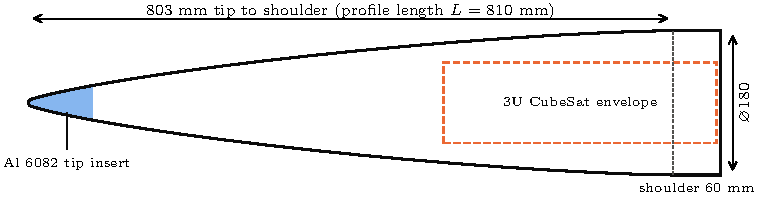
\includegraphics[width=\textwidth]{fig_final}
\caption{Selected nose cone to scale: Von K\'arm\'an profile, $L/D = 4.5$, \SI{4.5}{mm} spherical
Al 6082 tip, \SI{60}{mm} bonded shoulder; dashed: 3U CubeSat envelope.}
\label{fig:final}
\end{figure}

\begin{table}[H]
\centering
\caption{Nose cone definition (outer mould line and performance).}
\label{tab:final}
\small
\begin{tabular}{@{}>{\raggedright\arraybackslash}p{5.4cm}>{\raggedright\arraybackslash}p{10.1cm}@{}}
\toprule
Profile & Von K\'arm\'an (Haack series, $C = 0$):
$y = \dfrac{R}{\sqrt\pi}\sqrt{\theta-\tfrac12\sin 2\theta}$, $\theta=\arccos\!\left(1-\dfrac{2x}{L}\right)$ \\
Base diameter $D = 2R$ & \SI{180}{mm} \\
Profile length $L$ (to the theoretical apex) & \FINL{} ($L/D = 4.5$) \\
Tip & sphere $r_n = \SI{4.5}{mm}$, tangent at $x = $ \FINXT{}; apex truncated by \FINTRUNC{} \\
Physical curved length (tip to shoulder) & \FINLPHYS{} \\
Shoulder & \SI{60}{mm} cylinder, Al male coupler bonded inside (Firehorn design) \\
Angle to the body at the shoulder & $0^\circ$ (tangent) \\
Internal volume / wetted area & \FINVOL{} / \FINAREA{} \\
Shell & CFRP prepreg $[0/45/0]_{SO}$, \SI{1.2}{mm}, on a PET-CF male mould (Firehorn process); GFRP if the nose must be an RF window \\
Tip insert & Al 6082-T6, machined, threaded onto a bonded Al ring (Matterhorn/Firehorn concept), $\sim\SI{60}{g}$, replaceable \\
Estimated mass (shell + tip, without coupler) & \FINMASS{} \\
Nose CP (Barrowman, from the apex) & \FINXCP{}, $C_{N\alpha} = 2$ \\
3U inside the curved part & \FINTHREEU{}; the remaining \FINCYL{} of the 3U sits behind the shoulder \\
Nose wave drag $C_{D,\rm w}$ at $M = 1.2/1.4/1.6$ & \FINCDB{} / \FINCDC{} / \FINCDD{} (Euler at $L/D=4.5$, sharp apex; $+0.5$ to $+1.4\,\%$ with the tip) \\
Apogee (nominal, model) & \FINAPO{}, i.e.\ \FINDAPO{} vs.\ the LVS-length baseline; $M_{\max} = \FINMMAX$ \\
Static margin change vs.\ baseline & \FINDSM{} cal \\
Peak temperatures (envelope) & tip \TIPAL{}; shell inner face \SHELLENV{} \\
\bottomrule
\end{tabular}
\end{table}

The \SI{4.5}{mm} sphere replaces the theoretical apex and removes \FINTRUNC{} of length, hence the
\FINLPHYS{} physical curved length. A radius tolerance of $\pm\SI{0.5}{mm}$ moves $C_{D,\rm w}$ by
much less than 1\,\%; a step at the tip/shell joint matters more, because a forward-facing step acts
as a small blunt face with a local shock and heating peak. Keep it below \SI{0.2}{mm} and
forward-facing steps at zero.

\subsection{Manufacturing plan}

\begin{enumerate}[leftmargin=*,itemsep=2pt]
\item \textbf{Mould.} Male mould printed in PET-CF from the CAD (Firehorn process). The \SI{870}{mm}
part (curved length + shoulder) is longer than one print bed and is printed in three segments,
joined at $x \approx 330$ and \SI{600}{mm} where the radius changes slowly, aligned on a central rod,
sanded and sealed with release agent.
\item \textbf{Layup.} Prepreg $[0/45/0]_{SO}$ (\SI{1.2}{mm}), the Firehorn laminate. Plies are cut
from flat patterns and stop at $x \approx \SI{60}{mm}$ (radius about \SI{17}{mm}), which avoids the
ply pile-up at the apex reported on Firehorn. Two extra local plies cover the last \SI{100}{mm} of the
curved part and the shoulder, where the coupler is bonded.
\item \textbf{Tip.} Machined Al 6082-T6 insert covering the first \SI{80}{mm}, threaded onto an Al
ring bonded inside the shell at $x = \SI{60}{mm}$, flush with the shell within \SI{0.2}{mm}.
\item \textbf{Coupler.} Firehorn male glued coupler, scaled to \SI{180}{mm}, bonded on the
\SI{60}{mm} shoulder (2027\_C\_ST\_COUPLERS).
\item \textbf{Finish.} Sand and paint. Check the profile with a printed template (or a CMM) at
five stations against \texttt{nose\_profile\_final.csv}, tolerance $\pm\SI{0.5}{mm}$.
\end{enumerate}

\subsection{Mass budget}

\begin{table}[H]
\centering
\caption{Mass budget of the nose cone structure (without payload, payload bay and coupler).}
\label{tab:mass}
\small
\begin{tabular}{@{}lrl@{}}
\toprule
Item & Mass [g] & Basis \\
\midrule
CFRP shell, \SI{0.300}{m^2} at \SI{0.98}{kg/m^2} & 294 & Firehorn as-built areal density \\
Local reinforcement plies (last \SI{160}{mm}) & 35 & 2 plies over \SI{0.09}{m^2} \\
Al 6082-T6 tip insert & 60 & machined, hollowed \\
Bonded Al tip ring + fastener & 20 & estimate \\
Adhesive (tip ring, coupler) & 25 & estimate \\
Paint and filler & 15 & \SI{0.05}{kg/m^2} \\
\midrule
\textbf{Total} & \textbf{449} & \\
Proposed requirement & 500 & 11\,\% margin \\
\bottomrule
\end{tabular}
\end{table}

\subsection{CAD deliverables}

The tool of Appendix~\ref{app:scripts} writes the profile coordinates
(\texttt{nose\_profile\_final.csv}, 200 points, $x$ from the tip), watertight binary STL solids (mm,
$x$ from the tip, closed by a flat base) of the seven candidates at $L/D = 4.5$ and of the final
design (\texttt{nose\_vonkarman\_LD4.5\_rn4.5mm\_FINAL.stl}, volume within 0.05\,\% of the
analytical one), and a STEP solid of the final design (same name, \texttt{.step}) for CAD and the
Ansys runs of R6.
